\documentclass[12pt, a4paper]{article} 

\usepackage[slovak]{babel}
\usepackage[utf8]{inputenc}
\usepackage[T1]{fontenc}
\usepackage{geometry}
\usepackage{graphicx}
\usepackage{multirow}
\usepackage{caption}
\usepackage{subcaption}
\usepackage{hyperref}
\usepackage{ulem}
\usepackage{setspace}
\usepackage{afterpage}

\geometry{
	a4paper,
	margin=2.5cm,
	top=2cm,
	bottom=2cm
}

\begin{document}
\begin{titlepage}
    \hspace{0pt}
    \vfill
    \centering
    \Large Semestrálny projekt \\ 
    \vspace{0.2cm}
    \huge  Softvérový viacvrstvový prepínač \\
    \vspace{1.2cm}
    \large Miroslav Hájek \\[0.1cm]
	\normalsize \textit{Predmet: Prepínanie a smerovanie v IP sieťach (2021/22)} \\[0.1cm]
	Fakulta informatiky a informačných technológií, \\
	Slovenská technická univerzita v Bratislave
    \vfill
\end{titlepage}
\pagenumbering{gobble}
\newpage
\tableofcontents
\newpage
\pagenumbering{arabic}
\setcounter{page}{1}
\setstretch{1.25}

\section{Zadanie}
Navrhnite a implementujte softvérový viacvrstvový prepínač na základe znalostí získaných z predmetu Počítačové
a komunikačné siete (PKS). Pri spracovaní koncepcie návrhu prepínača uvažujte viacportový prepínač. Ako
výsledná implementácia postačuje riešenie s dvojportovým prepínačom (dve sieťové karty, port 1 a port 2),
pričom ovládanie sieťových rozhraní realizujte príslušnými paketovými ovládačmi. Prepínač navrhnite a
implementujte v jazyku C++ alebo C\# (ďalšími povolenými jazykmi sú Java alebo Python). Navrhnite prepínač tak,
aby spĺňal požiadavky z úloh 1-4.

\subsection{Úloha 1: Prepínacia tabuľka} 
Zobrazoval  prepínaciu tabuľku  vo formáte  MAC  adresa  –  číslo portu  –  aktuálny  časovač záznamu. Prepínač sa 
obsah  svojej  prepínacej tabuľky učí priebežne a aktuálny stav  zobrazuje  cez grafické používateľské  rozhranie 
(obsah sa automaticky aktualizuje, nie pomocou tlačidla). Umožnite vyčistiť prepínaciu tabuľku pomocou tlačidla. 
Časovač  pre  vypršanie  záznamov  nech je konfigurovateľný  (pozn.:  nezabudnite  ošetriť vytiahnutie  kábla, ako aj 
výmenu káblov medzi portami). 

\subsection{Úloha 2: Štatistiky}
Poskytoval štatistické informácie vrstvy 2 - 4 RM OSI o počte (prijatých/odoslaných) PDU na každom porte v smere 
IN aj OUT,  ktoré  budú  zreteľne  zobrazovať  správne  fungovanie prepínača.  Umožnite resetovať štatistické 
informácie. Štatistické informácie nech zobrazujú minimálne informácie o PDU  typu  Ethernet  II,  ARP,  IP,  TCP, 
UDP, ICMP, HTTP.

\subsection{Úloha 3: Filtrácia komunikácie}
Filtroval komunikáciu na 2. - 4.vrstve  RM  OSI  vrátane portov  transportnej  vrstvy  a  typov  ICMP  (bez  použitia 
vstavaných  PCAP funkcií filtrovania). Riešenie navrhnite  ako  zoznam  pravidiel  vyhodnocovaných sekvenčne tak, 
aby bolo možné naraz realizovať ľubovoľnú kombináciu filtrov. Napr. pre danú IP povoliť iba HTTP komunikáciu a 
zároveň pre danú MAC zakázať ''ping''. Umožnite aj kombináciu  zdrojových a cieľových MAC a IP  adries, príp. 
portov. Zobrazujte tabuľku zadaných pravidiel a umožnite ich aj jednotlivo odstraňovať. Filtre rozlišujte v smere 
''in/out'' na každom porte prepínača (takisto zohľadniť v návrhu). Napr. Host A sa nedostane von na web (HTTP), 
ale u neho bežiaci server nginx (HTTP) bude dostupný. 

\subsection{Úloha 4: Variant B: System Logging (Syslog)}
Implementácia Syslog klienta, pričom je potrebné:
\begin{enumerate}
\setlength\itemsep{0em}
\item Zabezpečiť aspoň 3 úrovne dôležitosti správ (severity level).
\item Umožniť nakonfigurovať prepínaču zdrojovú IP adresu, z ktorej sa budú správy odosielať. 
\item Nakonfigurovať IP adresu vzdialeného Syslog servera.
\item Zasielané správy musia obsahovať časovú pečiatku (angl. timestamp).
\item Zvoľte aspoň 5 činností  (descriptions), ktoré budete pomocou Syslog zaznamenávať (napr. ,,Zariadenie s 
MAC X sa premiestnilo z portu 1 na port 2'').
\end{enumerate} 
Syslog server bude aplikácia TFTPD32 bežiaca na niektorom počítači  (prípadne Networkers' Toolkit pre GNS3). 
Umožnite spustenie/zastavenie Syslog funkcionality na prepínači.

\section{Návrh riešenia}
Softvérový dvojportový prepínač je napísaný v jazyku C++11 so zachytávaním a zostavovaním rámcov realizovaných knižnicou \textit{PcapPlusPlus} 21.11\footnote{PcapPlusPlus: \url{https://pcapplusplus.github.io/}} nad \textit{libpcap} 1.10.1. Grafické používateľské rozhranie zabezpečuje knižnica \textit{wxWidgets} 3.0.5\footnote{wxWidgets: \url{https://www.wxwidgets.org/}}.
Testovacím prostredím je platforma Manjaro Linux 5.10. s emulátorom GNS3 verzie 2.2.29.

Program sa skompiluje zadaním nasledujúceho príkazu za predpokladu nainštalovaných požadovaných knižníc:
\begin{verbatim}
g++ -std=c++11 -O2 -Wall switch.cpp `wx-config --cxxflags --libs` \
    -lPcap++ -lPacket++ -lCommon++ -lpcap -lpthread \
    -I/usr/local/include/pcapplusplus -o switch
\end{verbatim}

Implementovaný softvérový prepínač predpokladá existenciu dvoch loopback rozhraní s názvami \verb|port1| a \verb|port2|, 
preto je ich nutné pred spustením vytvoriť a uviesť do stavu UP.
\begin{verbatim}
ip link add name port1 type dummy
ip link add name port2 type dummy
ip link set port1 up
ip link set port2 up
\end{verbatim}
Aby rozhrania umožnili preposlanie premávky musia byť považované za aktívne, tým že pravidelne prijímajú
keepalive správy (napr. v GNS rámce LOOP z Cisco routerov pripojených na hub alebo z počítačov s nekonečným ping-om.)
Po 5 sekundách neaktivity na rozhraní bude považované za odpojené.

\subsection{Prepínanie rámcov}
Viacportový prepínač (switch) narozdiel od rozbočovača (hub) zaznamenáva koncové zariadenia v LAN sieti 
dosiahnuteľné na aktívnych linkách v tabuľke MAC adries (ďalej označované CAM - Content Addressable Memory), 
z dôvodu adresnosti rozposielania rámcov do destinácie bez zbytočného zahltenia média pri oddelení kolíznych domén.

Po prijatí Ethernet rámca na ľubovoľnom rozhraní sa podľa cieľovej MAC adresy určí, ktorými ostatnými aktívnymi 
linkami dôjde k preposlaniu. L2 broadcast označený MAC adresou ff:ff:ff:ff:ff:ff bude propagovaný všetkými rozhraniami, 
rovnako ako rámec s cieľovou MAC adresou, ktorá ešte nie je v CAM tabuľke. Na známu MAC adresu sa rámec pošle najviac cez jedno 
rozhranie, ktoré je viazané s danou MAC adresou. Rámec sa nikdy nevráti rozhraním odkiaľ bol prijatý. 
\begin{figure}[h!]
	\centering
	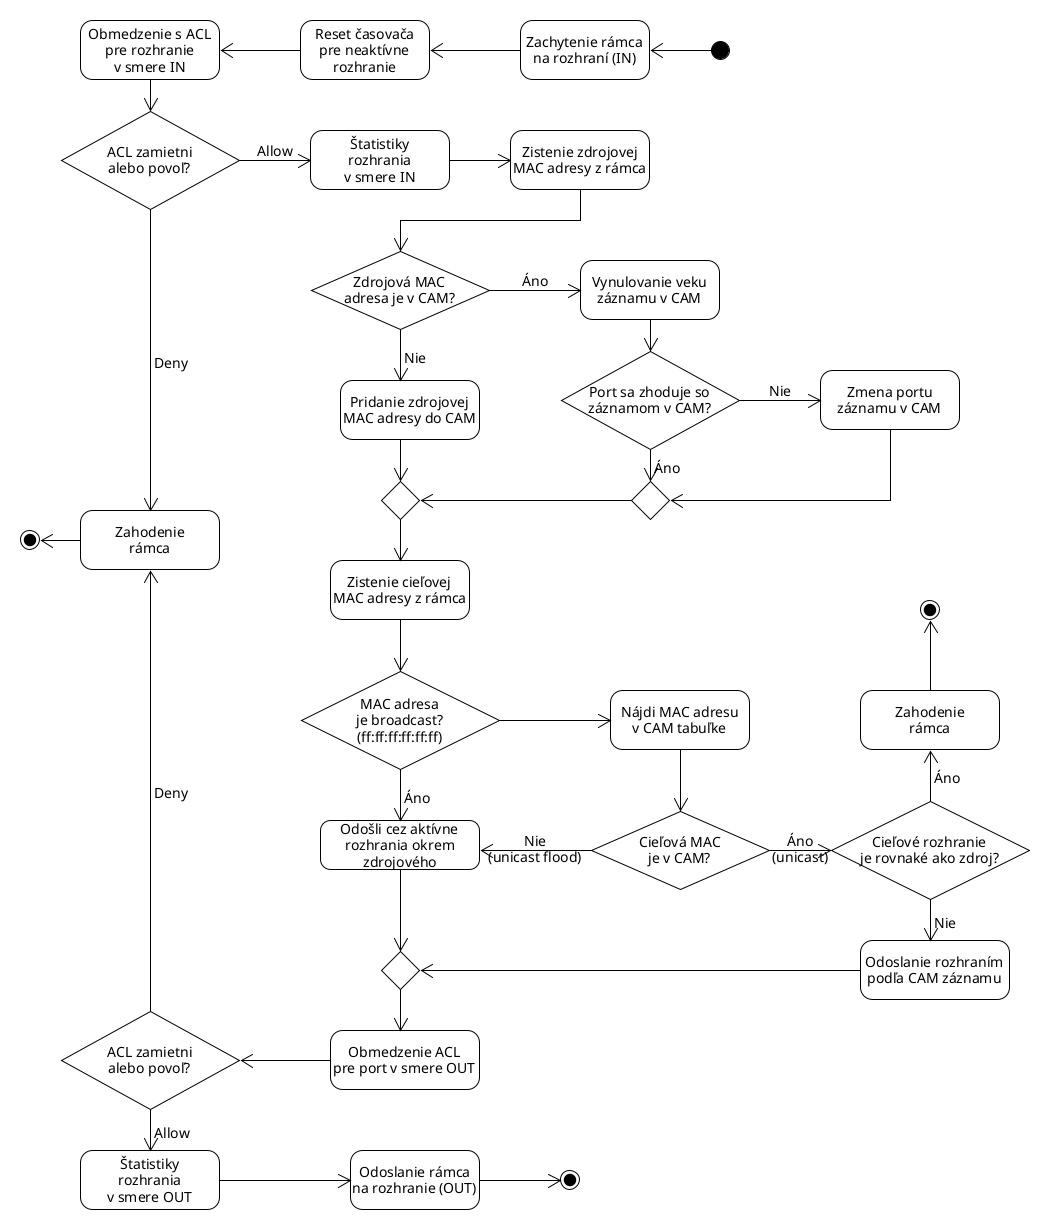
\includegraphics[width=0.9\textwidth]{assets/switch.png}
	\caption{Proces preposlania rámca na viacportovom prepínači}
\end{figure}
Na základe zdrojovej MAC adresy zisťuje prepínač, kde sú pripojené koncové zariadenia, čím vytvára záznamy v CAM tabuľke 
realizovanej hashovacou tabuľkou (\verb|std::unordered_map|). MAC adresa je asociovaná so štruktúrou obsahujúcou označenie 
prijímajúceho portu (poradové číslo) a vek záznamu v sekundách (age) inkrementovaný časovačom. 


Port záznamu sa zmení vtedy, ak je zdrojová MAC adresa videná na inom rozhraní. Vek záznamu sa vynuluje po objavení akéhokoľvek rámca zo 
zdroja. Záznam v CAM je zmazaný ak je asociovaný port neaktívny 5 sekúnd alebo vek záznamu je väčší ako hodnota časovača pre 
vypršanie záznamov nastavená v GUI.

Na zamedzenie cyklenia premávky sú rámce po prijatí serializovane uložené do množiny typu \verb|std::unordered_set|, z dôvodu 
nefunkčnosti filtrovania smeru na loopback rozhraniach s libpcap. Pri odosielaní na výstupný port je z množiny rámec zmazaný.

\begin{figure}[h!]
	\centering
	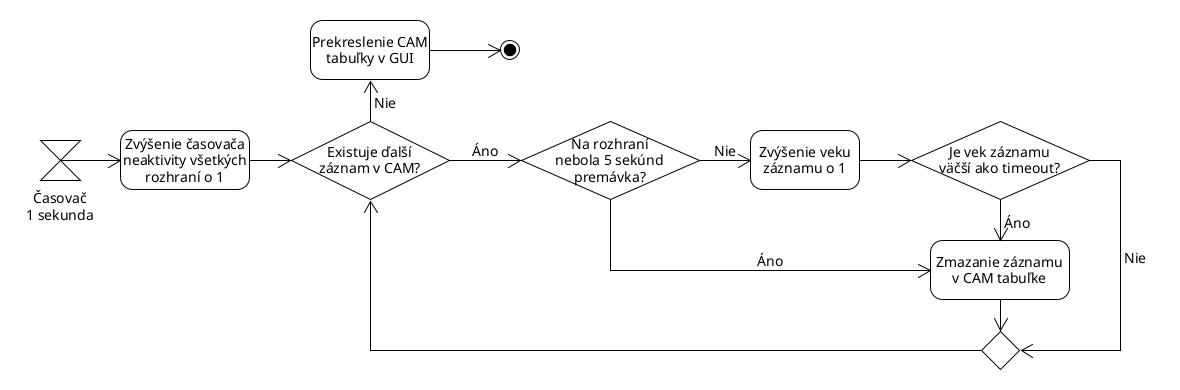
\includegraphics[width=\textwidth]{assets/mac-table.png}
\end{figure}

\subsection{Filtrácia premávky s ACL}
Zoznamy pre riadenie prístupu (Access-control list) na prepínači riadia povolenie (allow) alebo zakázanie (deny) vybranej premávky.
ACL sú nastaviteľné pre každé rozhranie prepínača nezávisle, zvlášť v smeroch príjmu (IN - inbound) aj vysielania (OUT - outbound). 
Pravidlá ACL pre kombináciu port a smer sú uložené v dynamickom poli (\verb|std::vector|) a sú vyhodnocované sekvenčne od prvého po 
posledné. Aplikovanie pravidiel v tabuľke v GUI nasleduje poradie zhora nadol.

Na zhodu vlastností rámca s pravidlom sa kontrolujú len vyplnené obmedzenia platné pre prítomné vnorené protokoly.
Pravidlo dokáže overiť zdrojovú a cieľovú MAC adresu, zdrojovú a cieľovú IPv4 a IPv6 adresu, zdrojový a cieľový
port, a filtrovaný protokol z výberu: TCP, UDP, ICMP Echo request (typ 8), ICMP Echo reply (typ 0). Pri zvolení protokolu 
ICMP nebude možné v rozhraní zadať port.

Prázdne políčka sú pri hľadaní zhody považované za platné vždy pre daný rámec (stav ,,any''). Na záver sa aplikuje implicitné povolenie 
premávky, ktorá nebola zakázaná predošlými pravidlami.
\begin{table}[t]
\begin{tabular}{|l|c|c|r|c|c|c|l|}
\hline
\textbf{Policy} & \multicolumn{1}{r|}{\textbf{Mac Src}}  & \multicolumn{1}{r|}{\textbf{Mac Dst}} & \textbf{IP Src}                   & \multicolumn{1}{r|}{\textbf{IP Dst}} & \multicolumn{1}{r|}{\textbf{Port Src}} & \multicolumn{1}{l|}{\textbf{Port Dst}} & \textbf{Protokol}             \\ \hline
\textbf{Allow}  & \textit{any}                           & \textit{any}                          & 1.1.1.2                           & \textit{any}                         & \textit{any}                           & 80                                     & TCP                                \\ \hline
\textbf{Deny}   & \textit{any}                           & \textit{any}                          & 1.1.1.2                           & any                                  & \textit{any}                           & any                                    & TCP \\ \hline
\textbf{Deny}   & \multicolumn{1}{r|}{aa:aa:...} & \textit{any}                          & \multicolumn{1}{c|}{\textit{any}} & any                                  & \textit{any}                           & any                                    & ICMP Echo reply                     \\ \hline
\end{tabular}
\caption{príklad na povolenie HTTP komunikácie na danej IP a zakázanie ,,ping'' na MAC adrese v smere IN na rozhraní pre PC}
\end{table}

\begin{figure}[t]
	\centering
	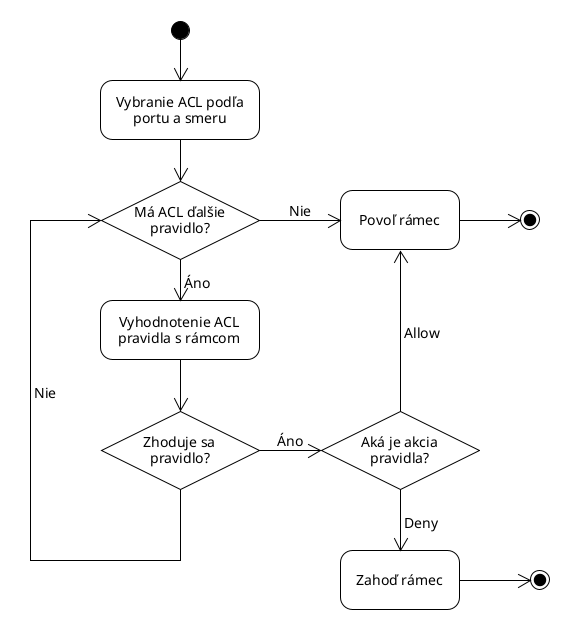
\includegraphics[width=0.6\textwidth]{assets/acl.png}
	\caption{Vyhodnotenie ACL pravidiel v jednom zozname pre kombináciu port a smer}
\end{figure}
\newpage

\subsection{Syslog protokol}
Syslog je štandard a aplikačný protokol nad UDP portom 514 slúžiaci na záznam hlásení o behu programov opísaný v RFC 5424.
Nezaručuje žiadne potvrdenie správ, ani nie je spojovo orientovaný, čím sa sled správ potrebný na zabezpečenie
komunikácie zužuje na jeden datagram v korektnom tvare odoslaný syslog serveru.

Rámec so syslog správou sa zostaví nasledovne: keďže nepoznáme priradenie MAC adries k IP adresám prostredníctvom ARP tabuľky, musel by 
byť rámec odoslaný s cieľovou broadcast MAC adresou všetkými rozhraniami prepínača. V implementácii budeme pre jednoduchosť topológie
poznať MAC adresu syslog servera, ktorá bude napevno určená v kóde. Zdrojová MAC adresa sa vyplní podľa MAC adresy konkrétneho loopback rozhrania, ktorou je rámec posielaný.

Zdrojová a cieľová IP adresa pre IP hlavičku musia byť pred spustením syslog služby nastavené cez GUI. V IP hlavičke sa vyplní
číslo protokolu na 17 pre UDP. Zdrojový aj cieľový UDP port sú 514, dĺžka datagramu sa určí podľa veľkosti posielanej správy.

\subsubsection{Štruktúra Syslog správy}
\begin{table}[]
\begin{tabular}{|l|l|l|l|l|l|l|l|l|l|l|l|l|l|l|l|}
\hline
\textbf{Priority}            & \textbf{Version} & \textbf{SP} & \textbf{Timestamp} & \textbf{SP} & \textbf{Hostname} & \textbf{SP} & ... \\ \hline
\textless{}134\textgreater{} & 1       & \textvisiblespace   & 2022-03-01T14:50Z &  \textvisiblespace  & SW1      & \textvisiblespace   & ...     \\ \hline
\end{tabular}
\end{table}

\begin{table}[]
\begin{tabular}{|l|l|l|l|l|l|l|l|l|}
\hline
\textbf{App} & \textbf{SP} & \textbf{Proc-ID} & \textbf{SP} & \textbf{Msg-ID} & \textbf{SP} & \textbf{Structured-Data} & \textbf{SP} & \textbf{Message} \\ \hline
          \textvisiblespace        &    \textvisiblespace         &      \textvisiblespace            &    \textvisiblespace         & Change          &             &                          &             & New MAC address             \\ \hline
\end{tabular}
\caption{Štruktúra Syslog správy podľa RFC 5424 s príkladom: facility = local0, severity = notice}
\end{table}

\begin{itemize}
\setlength\itemsep{0em}
\item \textbf{Priority} - pozostáva z 3 až 5 ASCII znakov. Vnútri špicatých zátvoriek ,,<'' a ,,>'' sa nachádza najviac trojciferné číslo priority v rozsahu 0 až 199. Číslo priority sa skladá z numerického kódu loggujúceho zariadenia (\textit{Facility}) 
vynásobeného 8 a sčítaného s číslom úrovne dôležitosti správy (\textit{Severity}). 

Facility v rozmedzí 0 - 15 sú priradené preddefinovaným systémovým službám, napr. 0 = správy kernelu, 2 = emailový systém, 3 = 
systémový daemony, 6 = subsystém tlačiarne apod. Na ľubovoľné využitie (local use) sú vyhradené facility local0 ... local7 s kódovým 
označením 16 - 23.

Severity umožňuje nastaviť 8 úrovní dôležitosti správ, od najdôležitejších s úrovňou 0 (Emergency) po najmenej dôležité s úrovňou 7
(Debug). Úrovne a ich účel sú nasledovné:
	\begin{enumerate}
		\setcounter{enumi}{0}
		\item Emergency: systém je nepoužiteľný
		\item Alert: vyžaduje sa okamžitá činnosť
		\item Critical: kritické podmienky
		\item Error: chybové podmienky
		\item Warning: varovanie
		\item Notice: normálne ale významné podmienky
		\item Informational: informačné správy
		\item Debug: správy na účely ladenia
	\end{enumerate}
\item \textbf{Version} - Verzia protokolu syslog zaevidovaná v IANA. Version = 1
\item \textbf{SP} - Označenie povinnej medzery ako oddelovača polí.
\item \textbf{Timestamp} - Časová pečiatka vo formáte ISO 8601. Oddelovač dátumu a času ,,T'' je povinný. Časový posun je povinný, buď vo časovej zóne UTC ,,Z'' alebo vyjadreným časovým posunom v hodinách '+01:00'. Rok - Mesiac - Deň ,,T'' Hodina : Minúta : Sekunda ,,Z''. Príklad: \textit{2022-03-01T12:25:10Z}.
\item \textbf{Hostname} - Doménové meno označujúce odosielateľa správy. Poradie preferencie pre hostname sú: plne kvalifikované doménové meno, statická IP adresa, doménové meno, dynamická IP adresa alebo ,,-''. Najviac 255 ASCII znakov.
\item \textbf{App} - Označenie zariadenia alebo aplikácie na účely filtrovania syslog správ. Prázdnou hodnotou je ,,-'' a často sa používa medzera ,, ''. Najviac 48 ASCII znakov.
\item \textbf{Proc-ID} - Nepovinné pole názvu alebo číslo procesu spojeného so syslog službou. Môže byť prázdne a najviac 128 ASCII znakov.
\item \textbf{Msg-ID} - Typ správy bez preddefinovaného významu. Môže byť prázdne a najviac 32 ASCII znakov.
\item \textbf{Structured-Data} - Nepovinné pole ponúkajúce spôsob formátovania údajov kľúč - hodnota. Element štruktúrovaných dát
je ohraničený hranatými zátvorkami. Element pozostáva z názvu vo formáte id@organizácia a aspoň jedného atribútu v tvare
key="value". Medzi viacerými elementami nesmie byť medzera. Vzorová správa riadiaca sa formátom pre Structured Data: \\
\verb|[mac@switch address="aa:bb:cc:dd:ee:ff" interface="port1"]|
\item \textbf{Message} - Voľný tvar textovej správy zakódovaný v UTF-8.
\end{itemize}

\subsubsection{Definovanie zaznamenávaných činností}
\begin{itemize}
\setlength\itemsep{0em}
\item (Informational) Device with MAC address X available on port Y.
\item (Informational) Timeout of record for device with MAC addresss X on port Y.
\item (Notice) Reset of CAM table
\item (Notice) Change of timeout for CAM records to X seconds.
\item (Warning) New ACL rule on port X in direction IN/OUT: Allow any any 1.1.1.1 ...
\item (Warning) Delete ACL rule on port X in direction IN/OUT: Allow any any 1.1.1.1 ...
\end{itemize}
\section*{Použité zdroje}
\begin{enumerate}
\item Configuring IP Access Lists. Cisco. \url{https://www.cisco.com/c/en/us/support/docs/security/ios-firewall/23602-confaccesslists.html}
\item RFC 5424. The Syslog Protocol. \url{https://www.rfc-editor.org/rfc/rfc5424.txt}
\item Analyze syslog messages with Seq.\url{https://blog.datalust.co/seq-input-syslog/}
\end{enumerate}
\newpage
\section{Grafické použivateľské rozhranie}
Rozhranie pozostáva zo štyroch obrazoviek v kartách podľa vykonávanej činnosti. Rozbaľovacie menu s názvom rozhrania alebo
smerom premávky pri štatistike premávky a filtrovaní ovplyvní zobrazenie zoznamu v tabuľke dole.
\begin{figure}[h!]
\centering
\begin{subfigure}{0.45\textwidth}
	\centering
	
\includegraphics[width=\textwidth]{assets/cam.png}
\end{subfigure}
\hfill
\begin{subfigure}{0.45\textwidth}
	\centering
	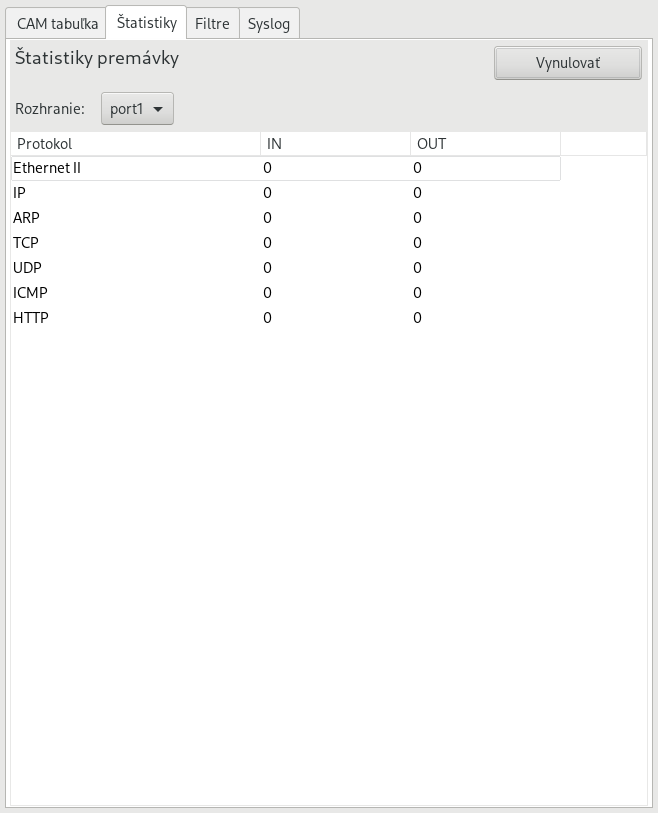
\includegraphics[width=\textwidth]{assets/stats.png}
\end{subfigure}
\hfill
\par\bigskip
\begin{subfigure}{0.45\textwidth}
	\centering
	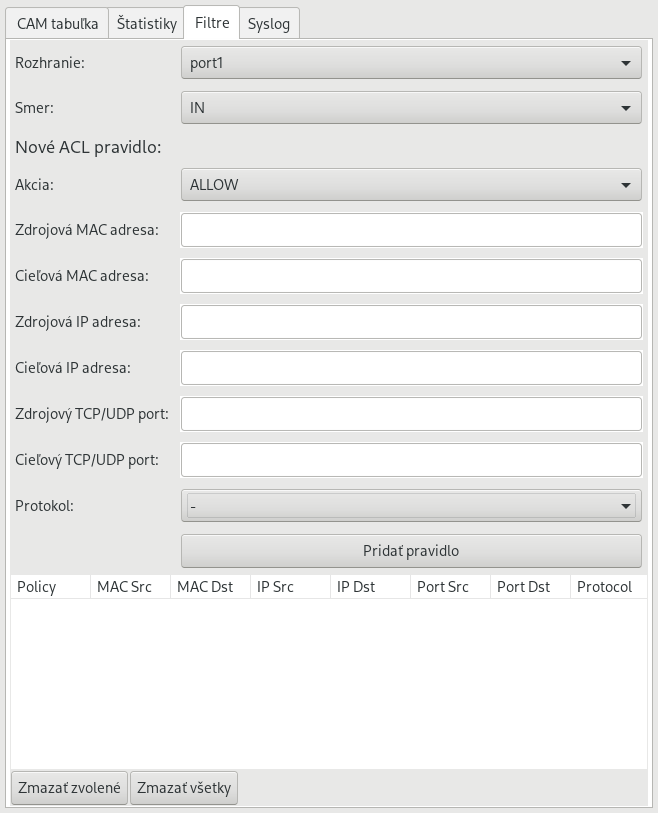
\includegraphics[width=\textwidth]{assets/filters.png}
\end{subfigure}
\hfill
\begin{subfigure}{0.45\textwidth}
	\centering
	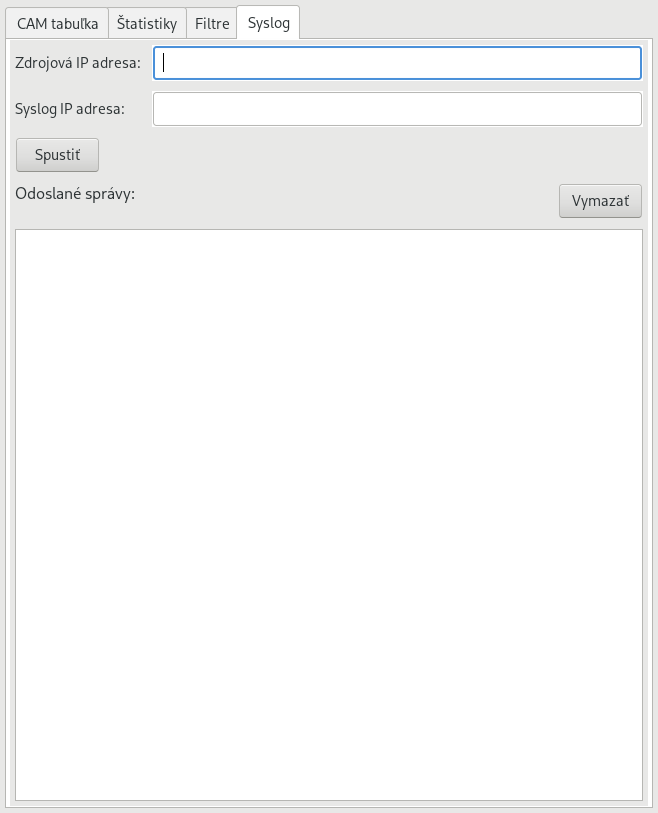
\includegraphics[width=\textwidth]{assets/syslog.png}
\end{subfigure}
\end{figure}


\end{document}